
{
    \newcommand{\tempwidth}[0]{0.8\linewidth}
    \begin{figure}
         \centering
         \begin{subfigure}{\textwidth}
             \centering
             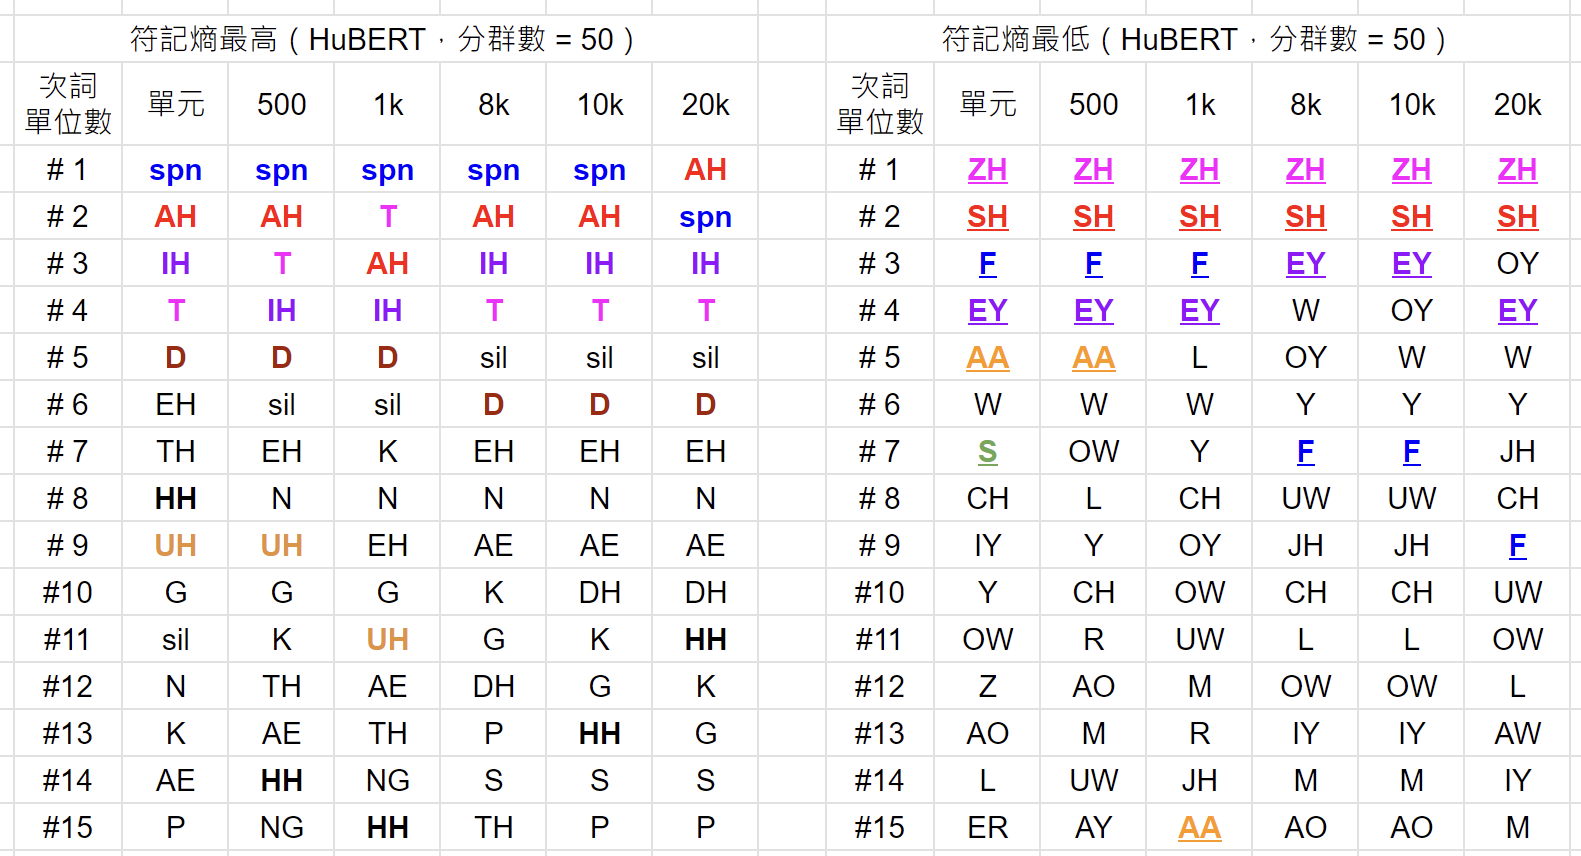
\includegraphics[width=\tempwidth]{figures/ch4figs/phnrank-hub50pcs.png}
             \caption{分群數 = 50}
             \label{fig:hub-u050-phnrank-hub50pcs}
         \end{subfigure}
         \vfill
         \begin{subfigure}{\textwidth}
             \centering
             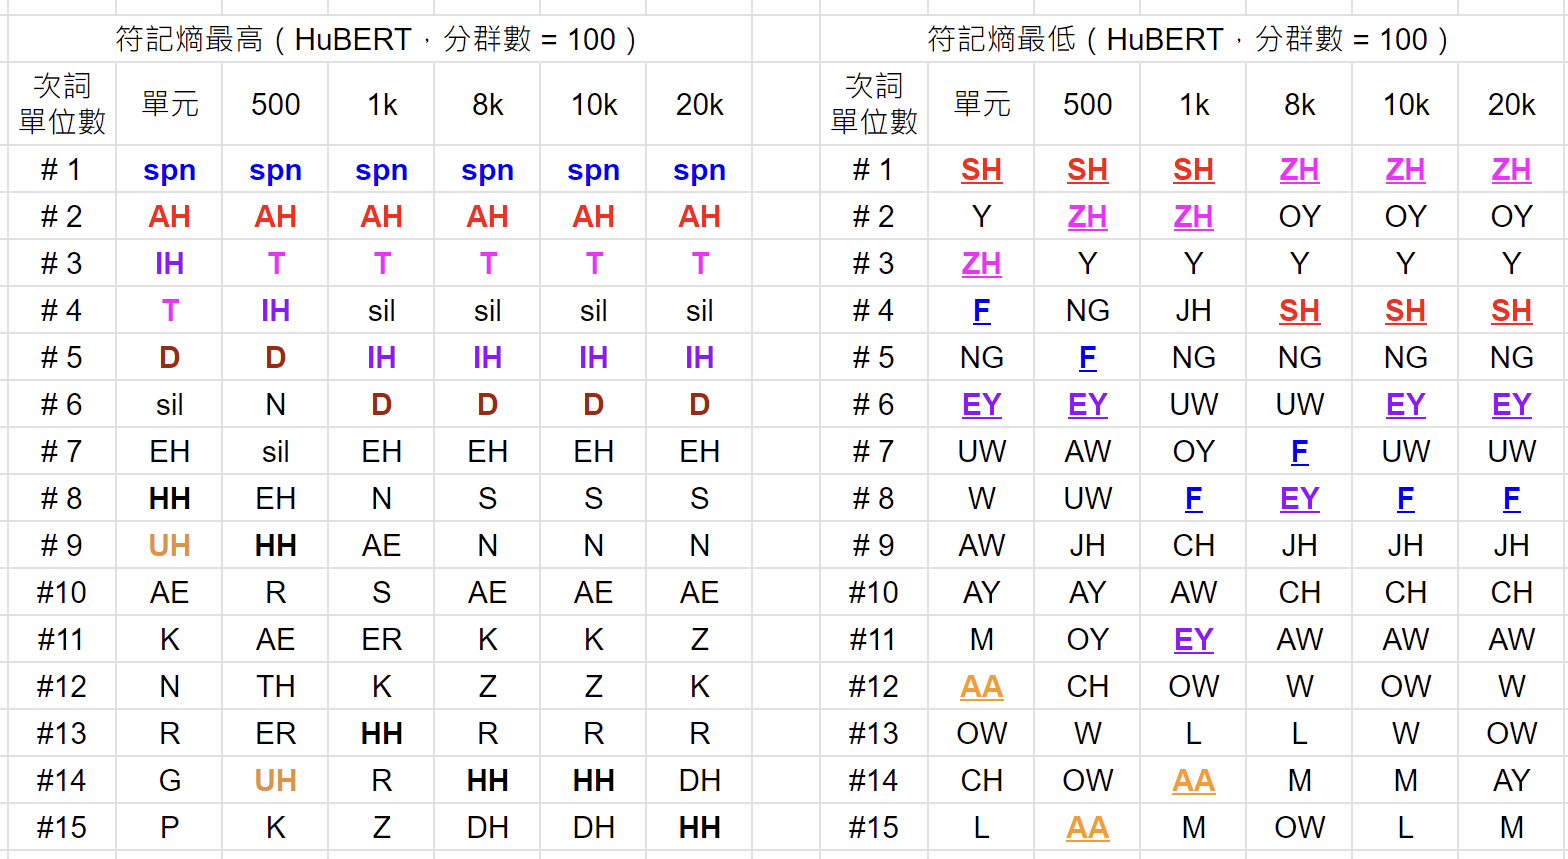
\includegraphics[width=\tempwidth]{figures/ch4figs/phnrank-hub100pcs.png}
             \caption{分群數 = 100}
             \label{fig:hub-u050-phnrank-hub100pcs}
         \end{subfigure}

         \caption{HuBERT 表徵、K-平均演算法分群數 50 和 100,}
         比較不同次詞單位種數時,符記熵最高與最低的音位排名
                     \label{fig:hub-u050-phnrank}
    \end{figure}
}

